% ~~~~~~~~~~~~~~~~~~~~~~~
% 
% AutoReportLite analysis pipeline & reporting template
% by Stephen Kelly
% April 29, 2016
%
% ~~~~~~~~~~~~~~~~~~~~~~~~
\documentclass[8pt]{beamer}\usepackage[]{graphicx}\usepackage[]{color}
%% maxwidth is the original width if it is less than linewidth
%% otherwise use linewidth (to make sure the graphics do not exceed the margin)
\makeatletter
\def\maxwidth{ %
  \ifdim\Gin@nat@width>\linewidth
    \linewidth
  \else
    \Gin@nat@width
  \fi
}
\makeatother

\definecolor{fgcolor}{rgb}{0.345, 0.345, 0.345}
\newcommand{\hlnum}[1]{\textcolor[rgb]{0.686,0.059,0.569}{#1}}%
\newcommand{\hlstr}[1]{\textcolor[rgb]{0.192,0.494,0.8}{#1}}%
\newcommand{\hlcom}[1]{\textcolor[rgb]{0.678,0.584,0.686}{\textit{#1}}}%
\newcommand{\hlopt}[1]{\textcolor[rgb]{0,0,0}{#1}}%
\newcommand{\hlstd}[1]{\textcolor[rgb]{0.345,0.345,0.345}{#1}}%
\newcommand{\hlkwa}[1]{\textcolor[rgb]{0.161,0.373,0.58}{\textbf{#1}}}%
\newcommand{\hlkwb}[1]{\textcolor[rgb]{0.69,0.353,0.396}{#1}}%
\newcommand{\hlkwc}[1]{\textcolor[rgb]{0.333,0.667,0.333}{#1}}%
\newcommand{\hlkwd}[1]{\textcolor[rgb]{0.737,0.353,0.396}{\textbf{#1}}}%

\usepackage{framed}
\makeatletter
\newenvironment{kframe}{%
 \def\at@end@of@kframe{}%
 \ifinner\ifhmode%
  \def\at@end@of@kframe{\end{minipage}}%
  \begin{minipage}{\columnwidth}%
 \fi\fi%
 \def\FrameCommand##1{\hskip\@totalleftmargin \hskip-\fboxsep
 \colorbox{shadecolor}{##1}\hskip-\fboxsep
     % There is no \\@totalrightmargin, so:
     \hskip-\linewidth \hskip-\@totalleftmargin \hskip\columnwidth}%
 \MakeFramed {\advance\hsize-\width
   \@totalleftmargin\z@ \linewidth\hsize
   \@setminipage}}%
 {\par\unskip\endMakeFramed%
 \at@end@of@kframe}
\makeatother

\definecolor{shadecolor}{rgb}{.97, .97, .97}
\definecolor{messagecolor}{rgb}{0, 0, 0}
\definecolor{warningcolor}{rgb}{1, 0, 1}
\definecolor{errorcolor}{rgb}{1, 0, 0}
\newenvironment{knitrout}{}{} % an empty environment to be redefined in TeX

\usepackage{alltt} % start LaTeX document
% set up parameters in R for use in the document

%


% ~~~~~~~~~~~~~~~~~~~~~~~~~~~~~~~~~~~~~~~~~~~~~~~~
% LaTeX settings start here:
\listfiles % get versions of files used for document compliaton, written at the end of the .log file for the report compilation!
\geometry{paperwidth=150mm,paperheight=105mm} % larger page size than normal for larger plots and more flexibility with font sizes
%\documentclass[8pt,xcolor={dvipsnames}]{beamer}
\setcounter{secnumdepth}{3} % how many levels deep before section headers stop getting numbers
\setcounter{tocdepth}{3} % table of contents depth
\usepackage{breakurl}
\usepackage{cite} % for citations, BibTeX I think
\usepackage{etoolbox} % this was not installed on HPCF, its in my home dir right now!! % has extra tools for LaTeX forloops, etc.; might not actually need this, use R loops to cat() LaTeX markup instead, much easier!
% \usepackage{forloop} % for LaTeX for loops; easier to use R loops to 'cat' TeX into the document instead!!
% \usepackage{tikz} % for custom graphics
%\usepackage{subcaption} %for subfigures%
% \usepackage{amsmath} % for math characters
\usepackage{graphicx} % good for advanced graphics options
\usepackage{tabularx} % for fancy table settings..
\usepackage{url} % for typesetting URLs, also file paths? 
\usepackage[multidot]{grffile} % support for image files with multiple '.' in the name
% \usepackage{adjustbox} % for auto-size box to put sample sheet into, also needs collectbox.sty
% \usepackage[usenames,dvipsnames]{color}
%%%%%%%%%%%%%experimental for xtable italics http://stackoverflow.com/questions/7996968/formatting-sweave-tables-two-challenges
% \usepackage{longtable} % allows for tables that break across pages
% \SweaveOpts{keep.source=TRUE}  % Keeps formatting of the R code.
%%%%%%%%%%%%%%%%%%%
%
% ~~~~~~ BEAMER SPECIFIC SETTINGS ~~~~~~~~ %
\makeatletter % turn on the '@' command character; needs to come before beamer settings
% \usetheme{Hannover} %  \usetheme{PaloAlto} % Bergen
% \usetheme[left]{Marburg} %  width= % hideothersubsections
\usetheme[left,hideothersubsections,width=3cm]{Marburg} %  width= % hideothersubsections
% location installed themes and such: /usr/share/texmf/tex/latex/beamer
\addtobeamertemplate{navigation symbols}{}{ % % this adds the page numbers at the bottom of the slide
    \usebeamerfont{footline}%
    \usebeamercolor[fg]{footline}%
    \hspace{1em}%
    \insertframenumber/\inserttotalframenumber
}
\makeatother % turn off the '@' command character; needs to come after beamer settings
% ~~~~~~~~~~~~~~~~~~~~~~~~~~~~~~~~~~~~~~~~~~~~%
% \graphicspath{/home/varitint/Dropbox/Lab/Teaching/Genomics_Class/Genomics_Lesson3_R!/With_embedded_R_code/figure/} % default path to find figures
%
%%%%%%%%%%
\IfFileExists{upquote.sty}{\usepackage{upquote}}{}
\begin{document}
% Create the Title page
\title[Sample Statistical Analysis]{SmithLab\_Taylor\_2016-12-31 Sample Statistical Analysis \\ Quality Metrics}
\author{Stephen Kelly}
\institute{\normalsize Dr. Aristotelis Tsirigos \\ PI: Dr. Smith \\ Genome Technology Center, \\ NYU Langone Medical Center, New York, NY 10016}
\date{\texttt{stephen.kelly@nyumc.org} \\ \today}
\titlegraphic{
\includegraphics[width=0.25\textwidth]{figure/NYULMC_white}} % image to show on the title slide
\maketitle

% REPORT STARTS HERE!
%
\section{Sample Sheet}
\begin{frame}{ Analysis Sample Sheet}
% latex table generated in R 3.2.3 by xtable 1.8-2 package
% Wed May  4 17:13:42 2016
\begin{table}[ht]
\centering
\begingroup\footnotesize
\scalebox{1.3}{
\begin{tabular}{rlll}
  \hline
 & SampleID & Control & genome \\ 
  \hline
1 & Sample1 & Sample2 & mm10 \\ 
  2 & Sample2 &  & mm10 \\ 
  3 & Sample3 & Sample4 & mm10 \\ 
  4 & Sample4 &  & mm10 \\ 
  5 & Sample5 &  & mm10 \\ 
   \hline
\end{tabular}
}
\endgroup
\end{table}
\end{frame}



\section{Sample1}
\subsubsection{Stats}
\begin{frame}{Stats }
\small{
Sample1 

Some sample stats

[1] -4.00 -3.99 -3.98 -3.97 -3.96 -3.95

[1] 0.0001338302 0.0001392850 0.0001449476 0.0001508253 0.0001569256

[6] 0.0001632564

[1] 3.167124e-05 3.303665e-05 3.445763e-05 3.593632e-05 3.747488e-05

[6] 3.907560e-05

[1]  1.2582925  0.6447519  0.4633460  0.7703058 -0.2263347 -0.3515479
}

\end{frame}

\subsubsection{distribution\_histogram.pdf}
\begin{frame}{distribution\_histogram.pdf }
\scriptsize{/ifs/home/kellys04/AutoReportLite/analysis\_pipeline/Sample1/Sample1.distribution\_histogram.pdf}
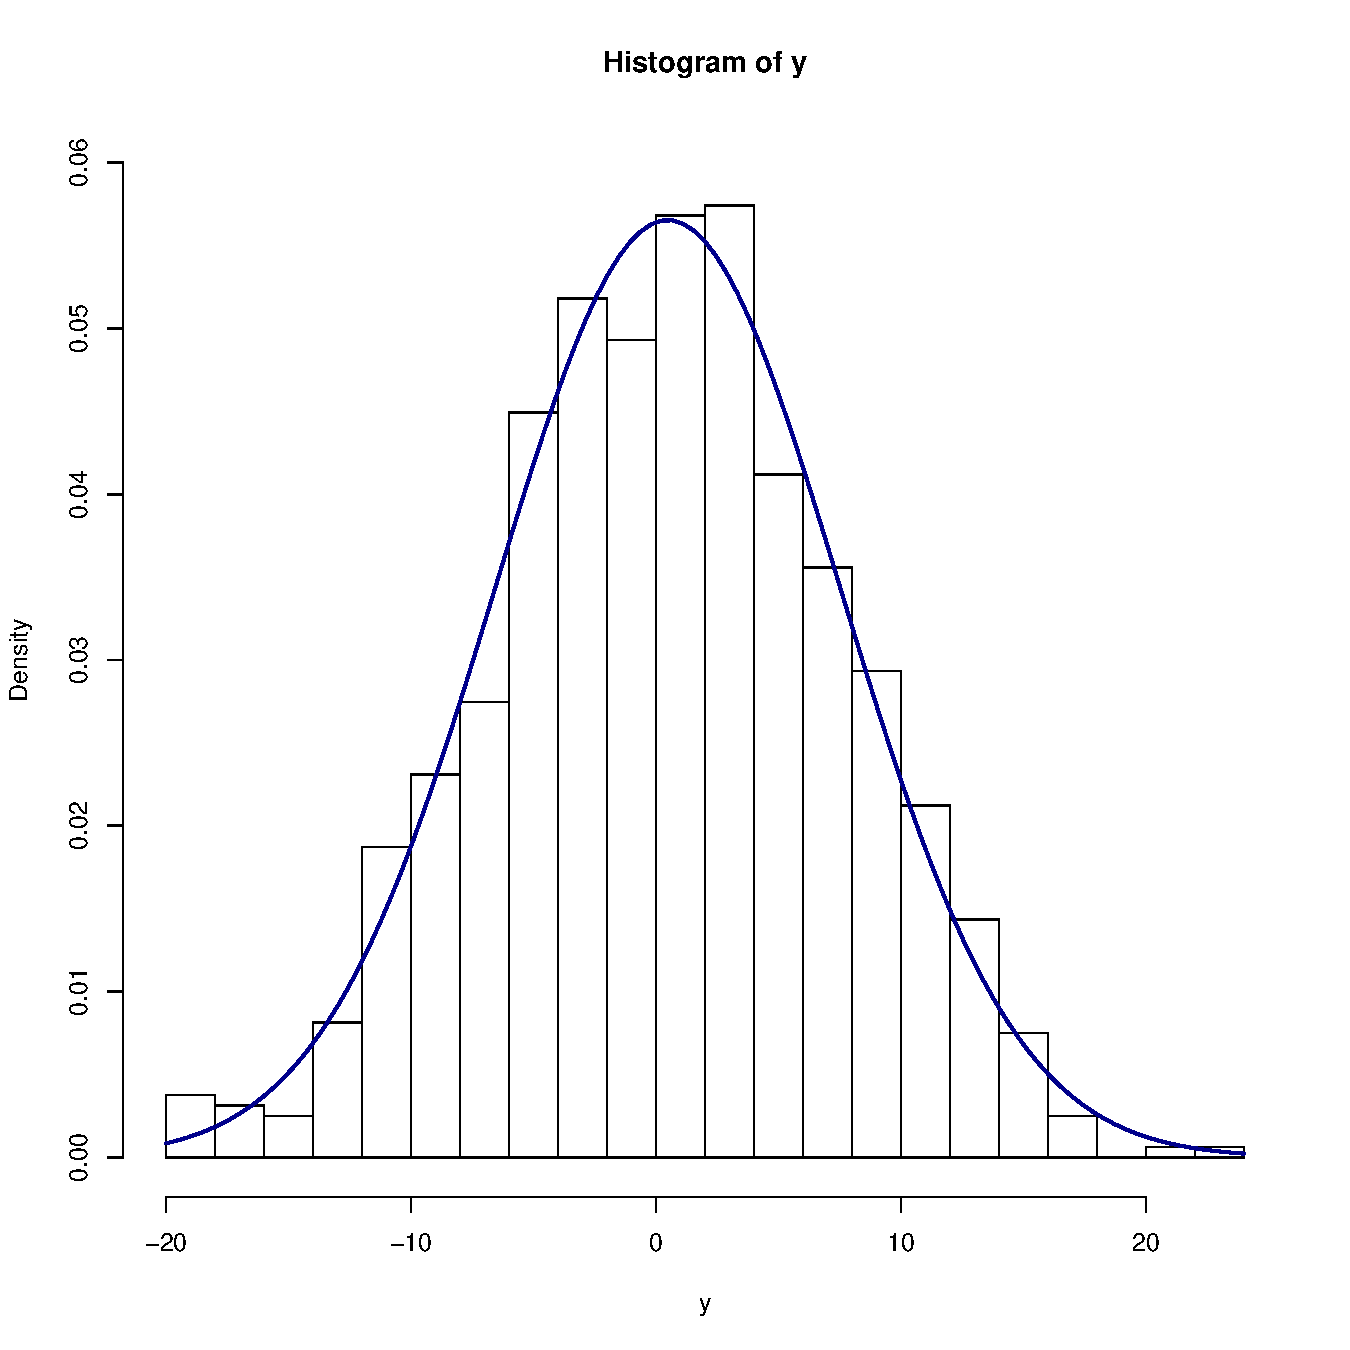
\includegraphics[width=0.9\linewidth,height=0.9\textheight,keepaspectratio]{/ifs/home/kellys04/AutoReportLite/analysis_pipeline/Sample1/Sample1.distribution_histogram.pdf}
\end{frame}

\subsubsection{random\_distribution.pdf}
\begin{frame}{random\_distribution.pdf }
\scriptsize{/ifs/home/kellys04/AutoReportLite/analysis\_pipeline/Sample1/Sample1.random\_distribution.pdf}
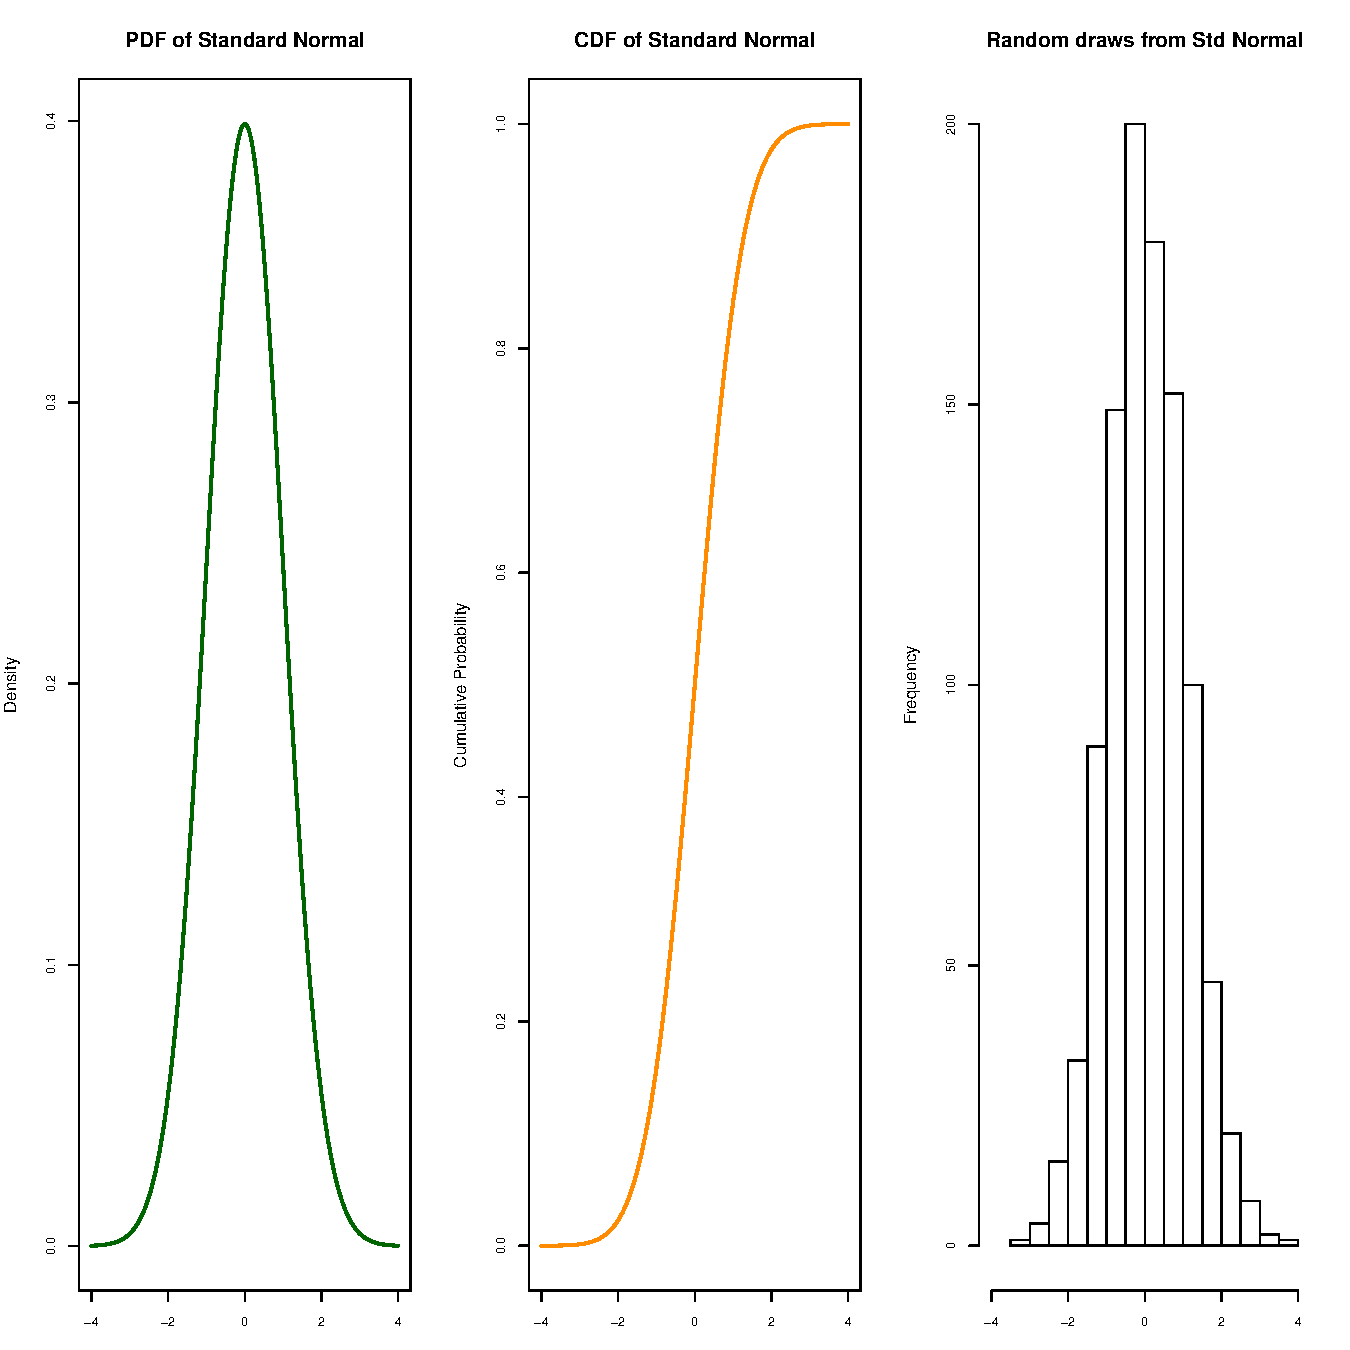
\includegraphics[width=0.9\linewidth,height=0.9\textheight,keepaspectratio]{/ifs/home/kellys04/AutoReportLite/analysis_pipeline/Sample1/Sample1.random_distribution.pdf}
\end{frame}

\section{Sample2}
\subsubsection{Stats}
\begin{frame}{Stats }
\small{
Sample2 

Some sample stats

[1] -4.00 -3.99 -3.98 -3.97 -3.96 -3.95

[1] 0.0001338302 0.0001392850 0.0001449476 0.0001508253 0.0001569256

[6] 0.0001632564

[1] 3.167124e-05 3.303665e-05 3.445763e-05 3.593632e-05 3.747488e-05

[6] 3.907560e-05

[1]  1.2582925  0.6447519  0.4633460  0.7703058 -0.2263347 -0.3515479
}

\end{frame}

\subsubsection{distribution\_histogram.pdf}
\begin{frame}{distribution\_histogram.pdf }
\scriptsize{/ifs/home/kellys04/AutoReportLite/analysis\_pipeline/Sample2/Sample2.distribution\_histogram.pdf}
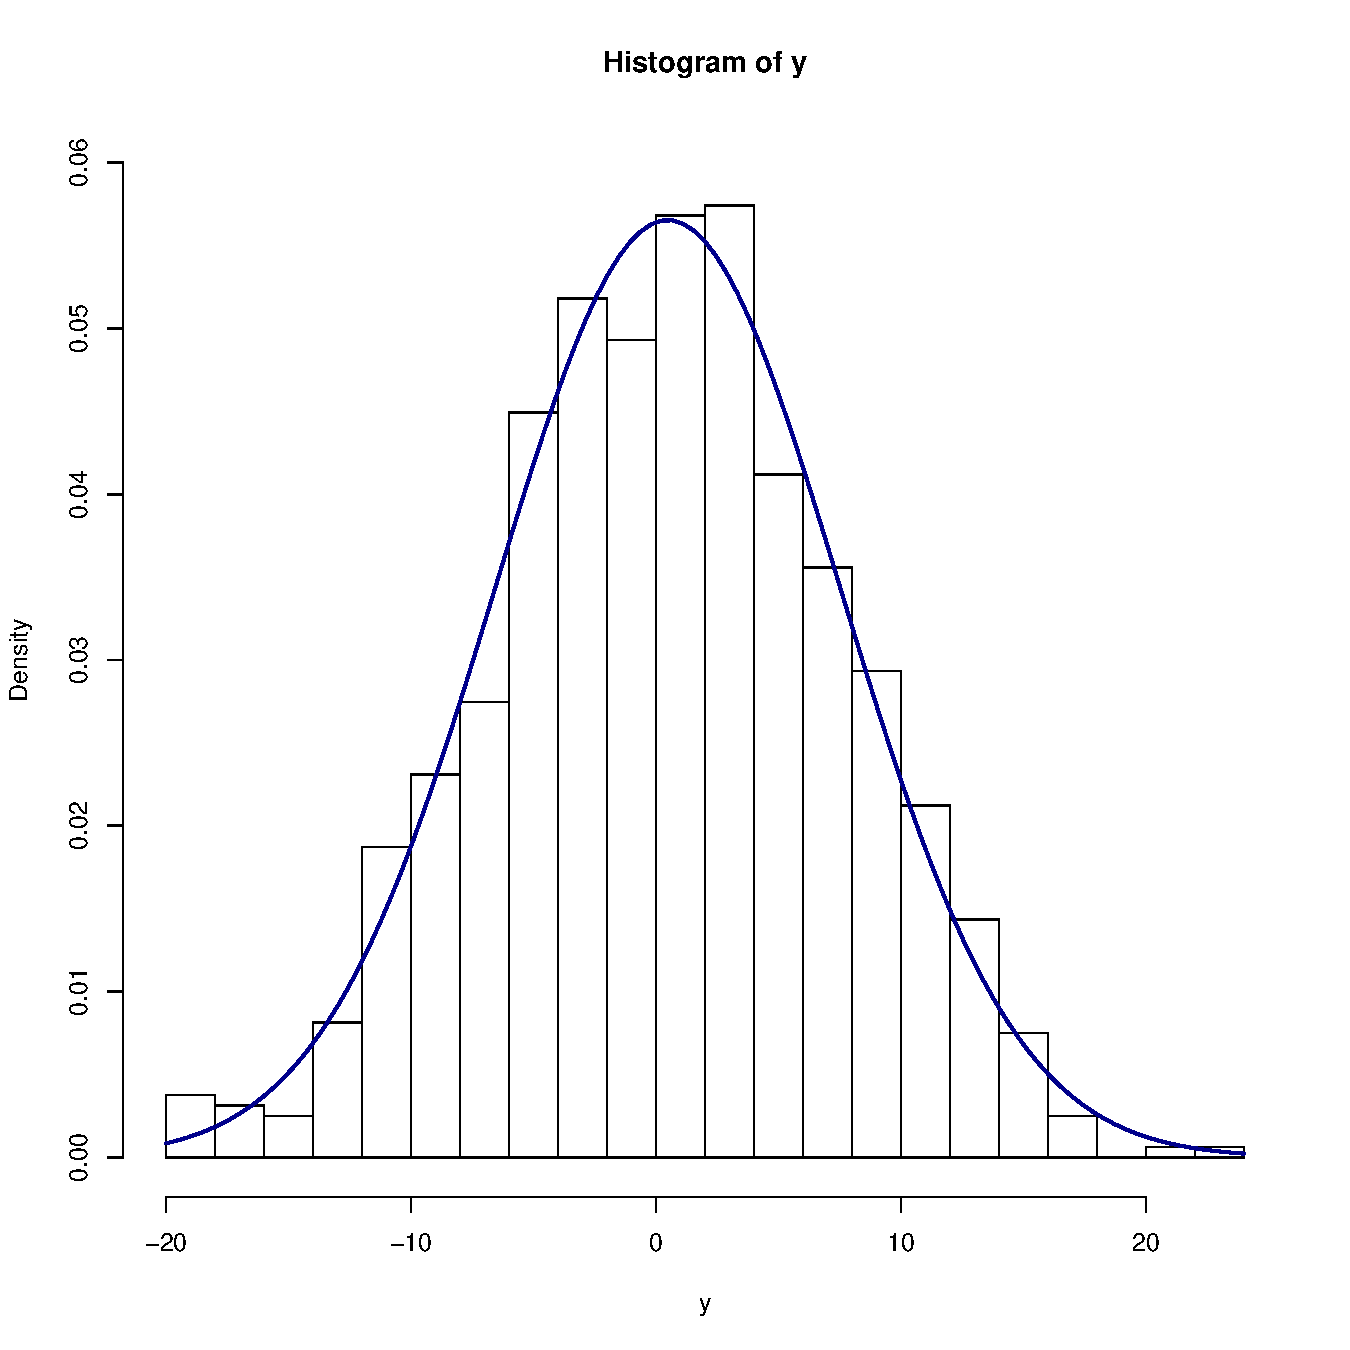
\includegraphics[width=0.9\linewidth,height=0.9\textheight,keepaspectratio]{/ifs/home/kellys04/AutoReportLite/analysis_pipeline/Sample2/Sample2.distribution_histogram.pdf}
\end{frame}

\subsubsection{random\_distribution.pdf}
\begin{frame}{random\_distribution.pdf }
\scriptsize{/ifs/home/kellys04/AutoReportLite/analysis\_pipeline/Sample2/Sample2.random\_distribution.pdf}
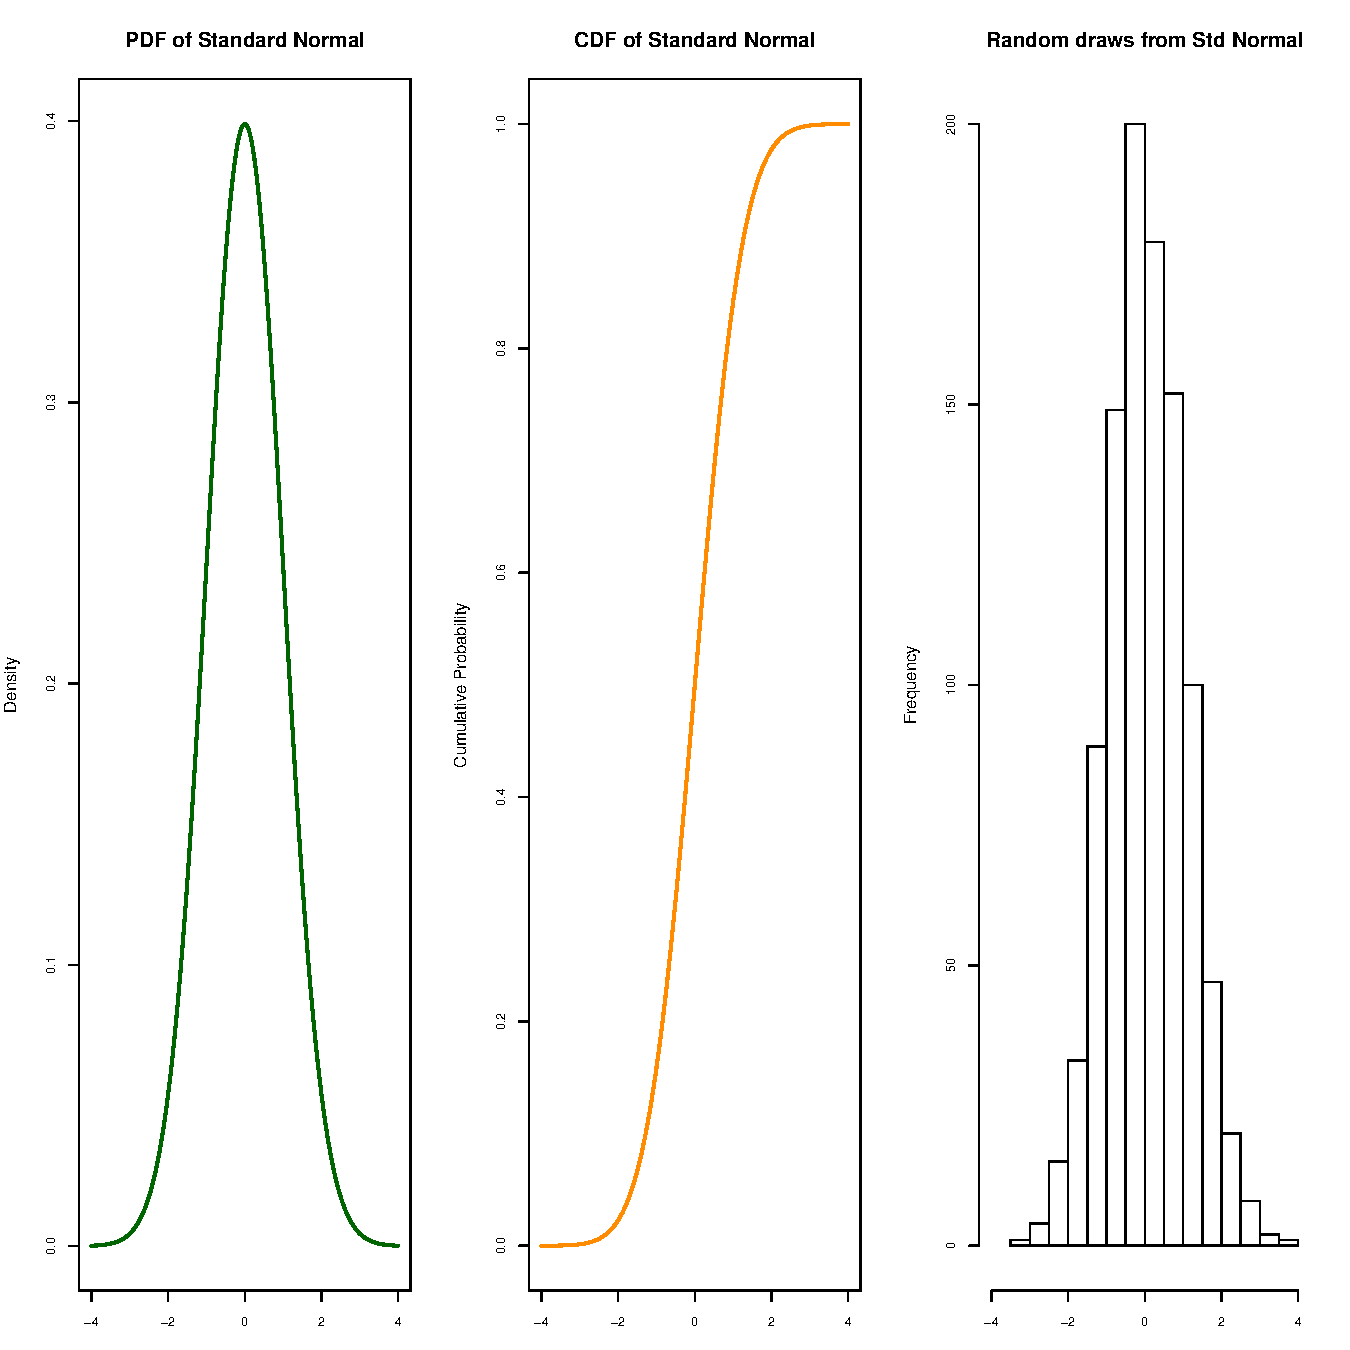
\includegraphics[width=0.9\linewidth,height=0.9\textheight,keepaspectratio]{/ifs/home/kellys04/AutoReportLite/analysis_pipeline/Sample2/Sample2.random_distribution.pdf}
\end{frame}

\section{Sample3}
\subsubsection{Stats}
\begin{frame}{Stats }
\small{
Sample3 

Some sample stats

[1] -4.00 -3.99 -3.98 -3.97 -3.96 -3.95

[1] 0.0001338302 0.0001392850 0.0001449476 0.0001508253 0.0001569256

[6] 0.0001632564

[1] 3.167124e-05 3.303665e-05 3.445763e-05 3.593632e-05 3.747488e-05

[6] 3.907560e-05

[1]  1.2582925  0.6447519  0.4633460  0.7703058 -0.2263347 -0.3515479
}

\end{frame}

\subsubsection{distribution\_histogram.pdf}
\begin{frame}{distribution\_histogram.pdf }
\scriptsize{/ifs/home/kellys04/AutoReportLite/analysis\_pipeline/Sample3/Sample3.distribution\_histogram.pdf}
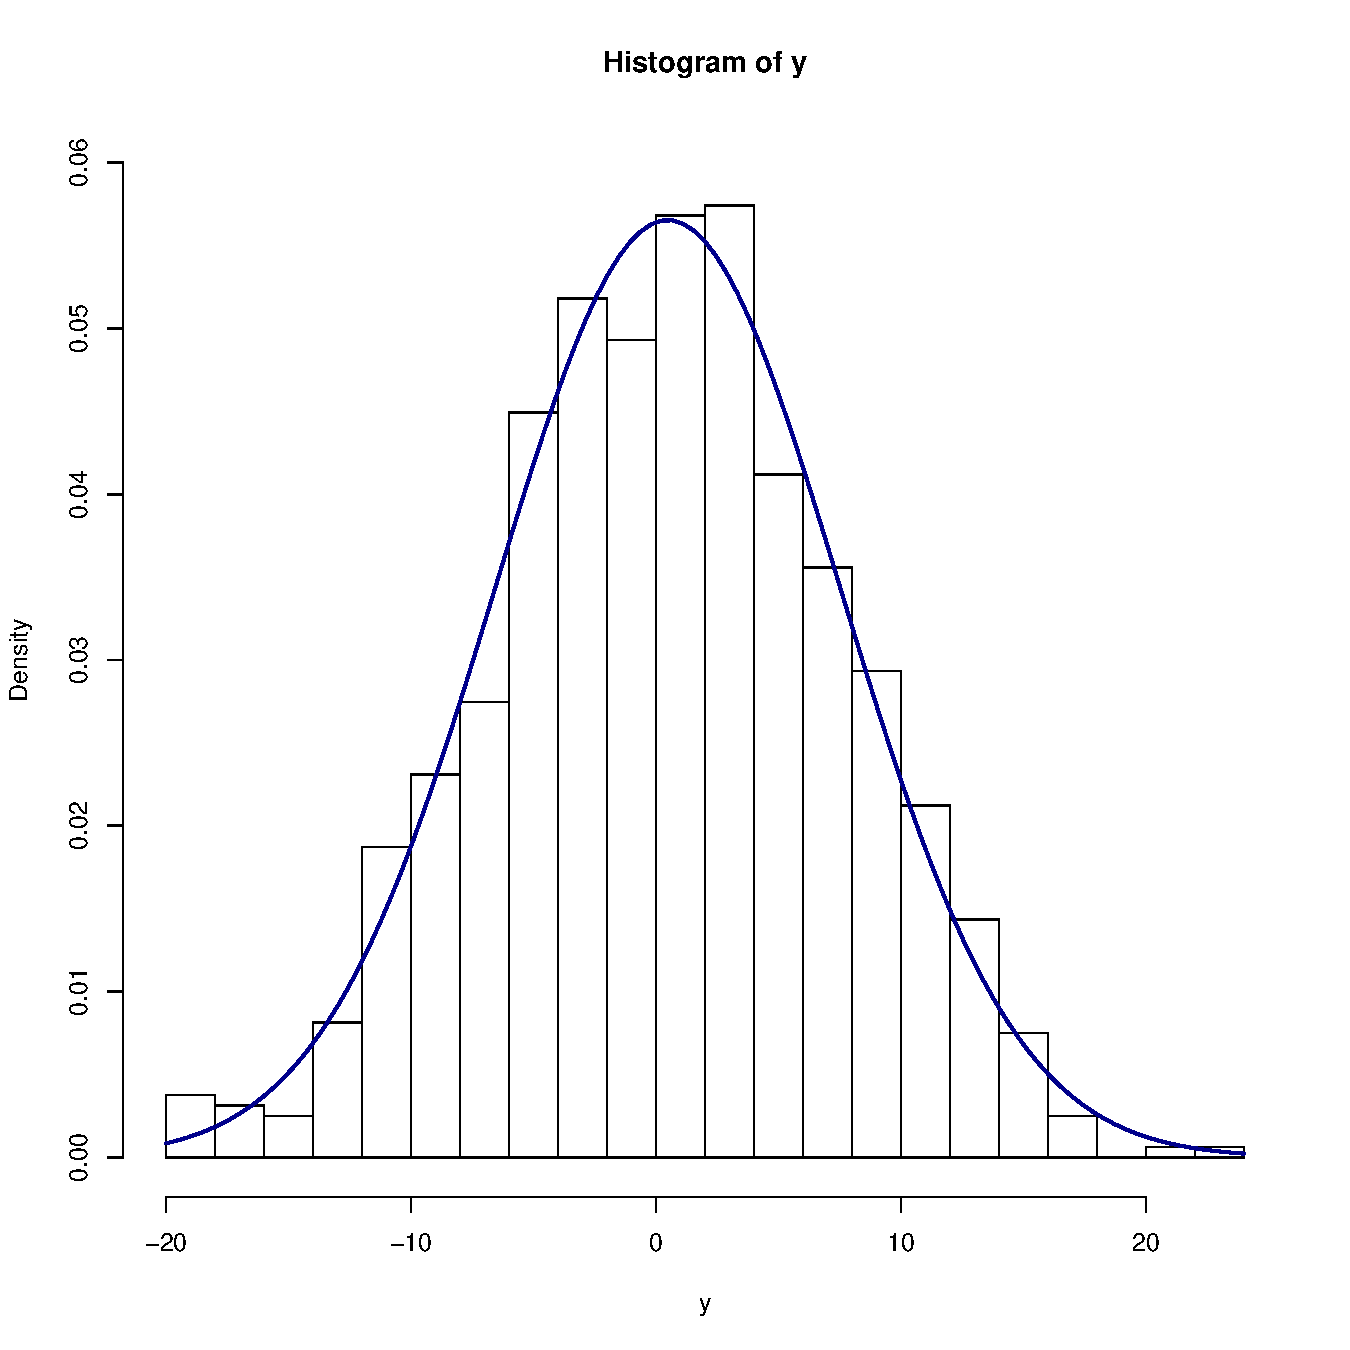
\includegraphics[width=0.9\linewidth,height=0.9\textheight,keepaspectratio]{/ifs/home/kellys04/AutoReportLite/analysis_pipeline/Sample3/Sample3.distribution_histogram.pdf}
\end{frame}

\subsubsection{random\_distribution.pdf}
\begin{frame}{random\_distribution.pdf }
\scriptsize{/ifs/home/kellys04/AutoReportLite/analysis\_pipeline/Sample3/Sample3.random\_distribution.pdf}
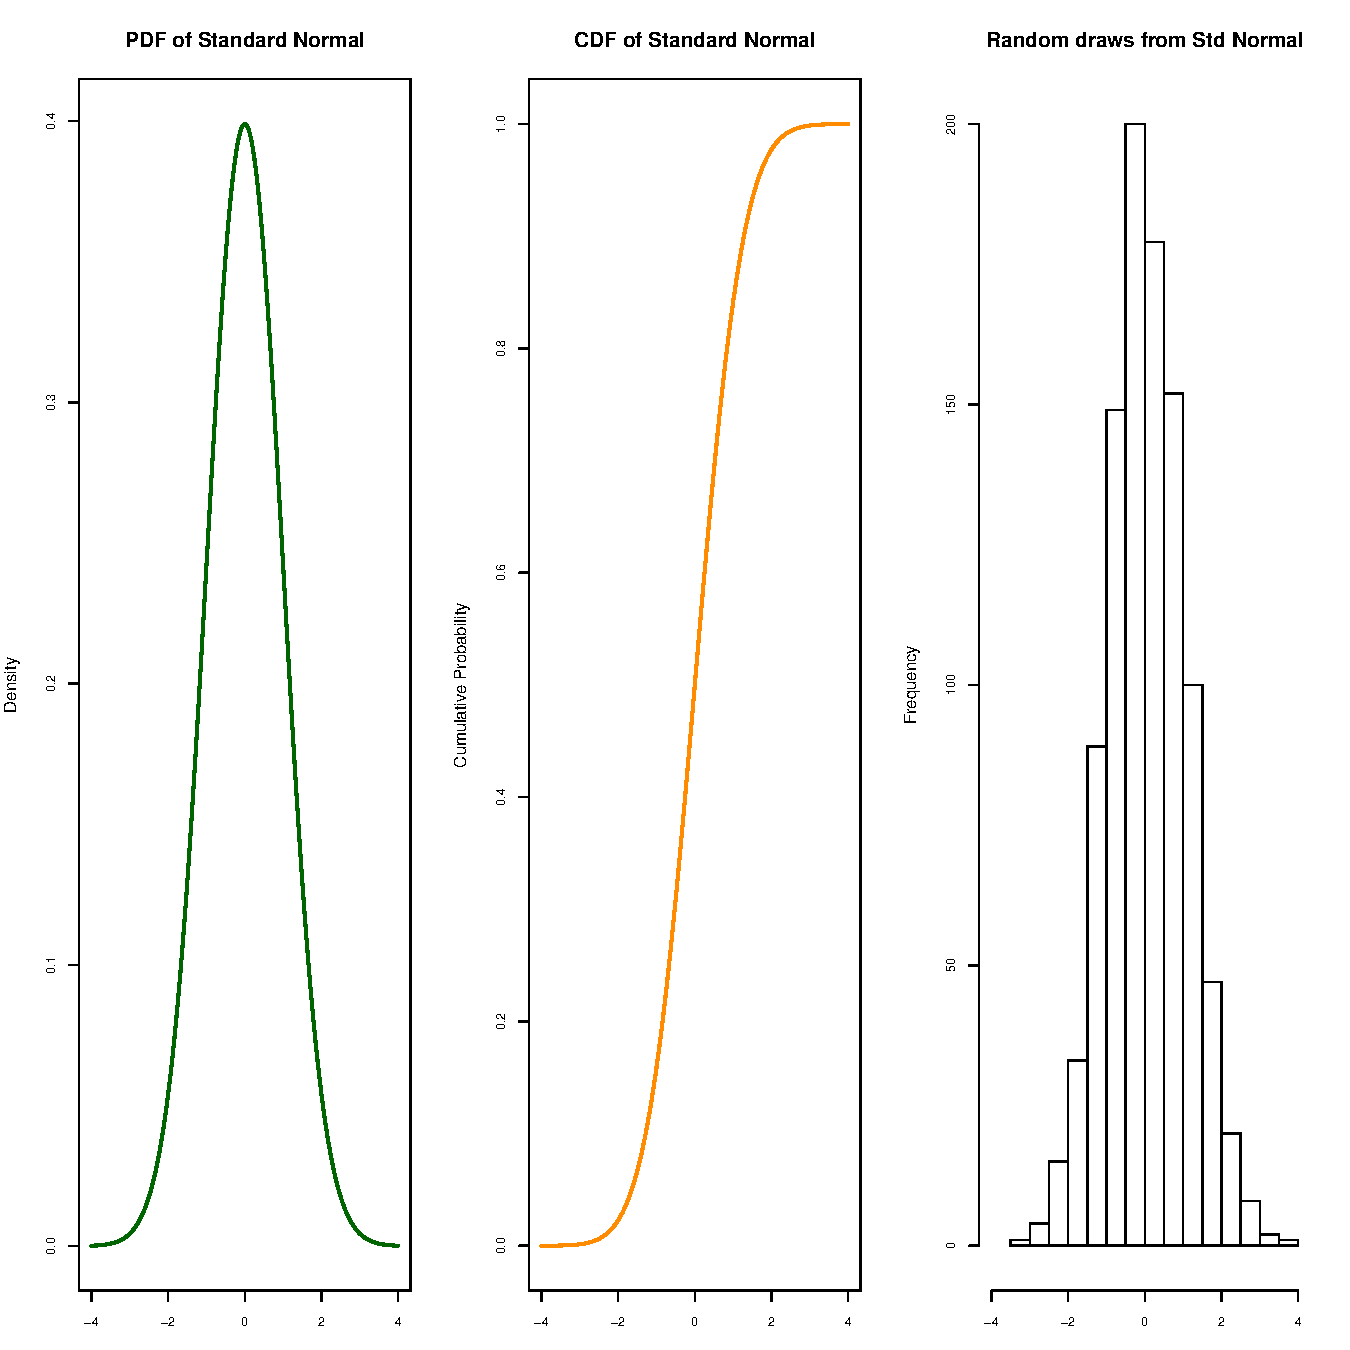
\includegraphics[width=0.9\linewidth,height=0.9\textheight,keepaspectratio]{/ifs/home/kellys04/AutoReportLite/analysis_pipeline/Sample3/Sample3.random_distribution.pdf}
\end{frame}

\section{Sample4}
\subsubsection{Stats}
\begin{frame}{Stats }
\small{
Sample4 

Some sample stats

[1] -4.00 -3.99 -3.98 -3.97 -3.96 -3.95

[1] 0.0001338302 0.0001392850 0.0001449476 0.0001508253 0.0001569256

[6] 0.0001632564

[1] 3.167124e-05 3.303665e-05 3.445763e-05 3.593632e-05 3.747488e-05

[6] 3.907560e-05

[1]  1.2582925  0.6447519  0.4633460  0.7703058 -0.2263347 -0.3515479
}

\end{frame}

\subsubsection{distribution\_histogram.pdf}
\begin{frame}{distribution\_histogram.pdf }
\scriptsize{/ifs/home/kellys04/AutoReportLite/analysis\_pipeline/Sample4/Sample4.distribution\_histogram.pdf}
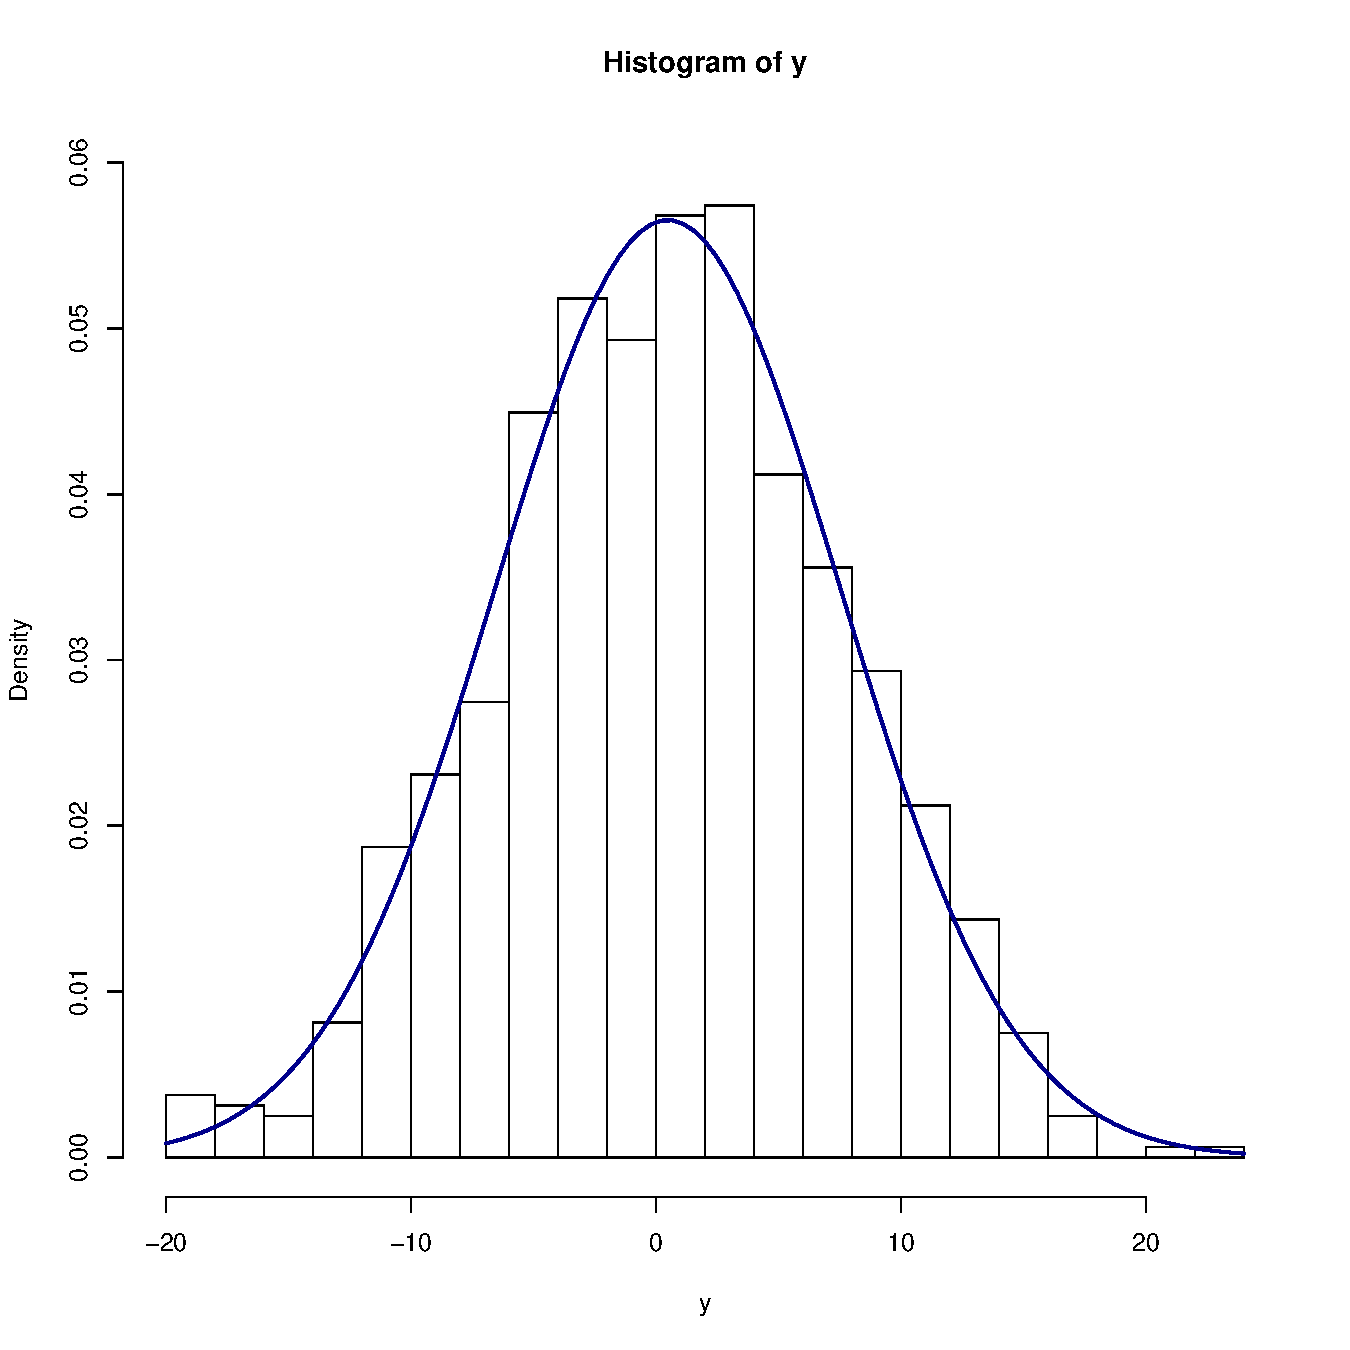
\includegraphics[width=0.9\linewidth,height=0.9\textheight,keepaspectratio]{/ifs/home/kellys04/AutoReportLite/analysis_pipeline/Sample4/Sample4.distribution_histogram.pdf}
\end{frame}

\subsubsection{random\_distribution.pdf}
\begin{frame}{random\_distribution.pdf }
\scriptsize{/ifs/home/kellys04/AutoReportLite/analysis\_pipeline/Sample4/Sample4.random\_distribution.pdf}
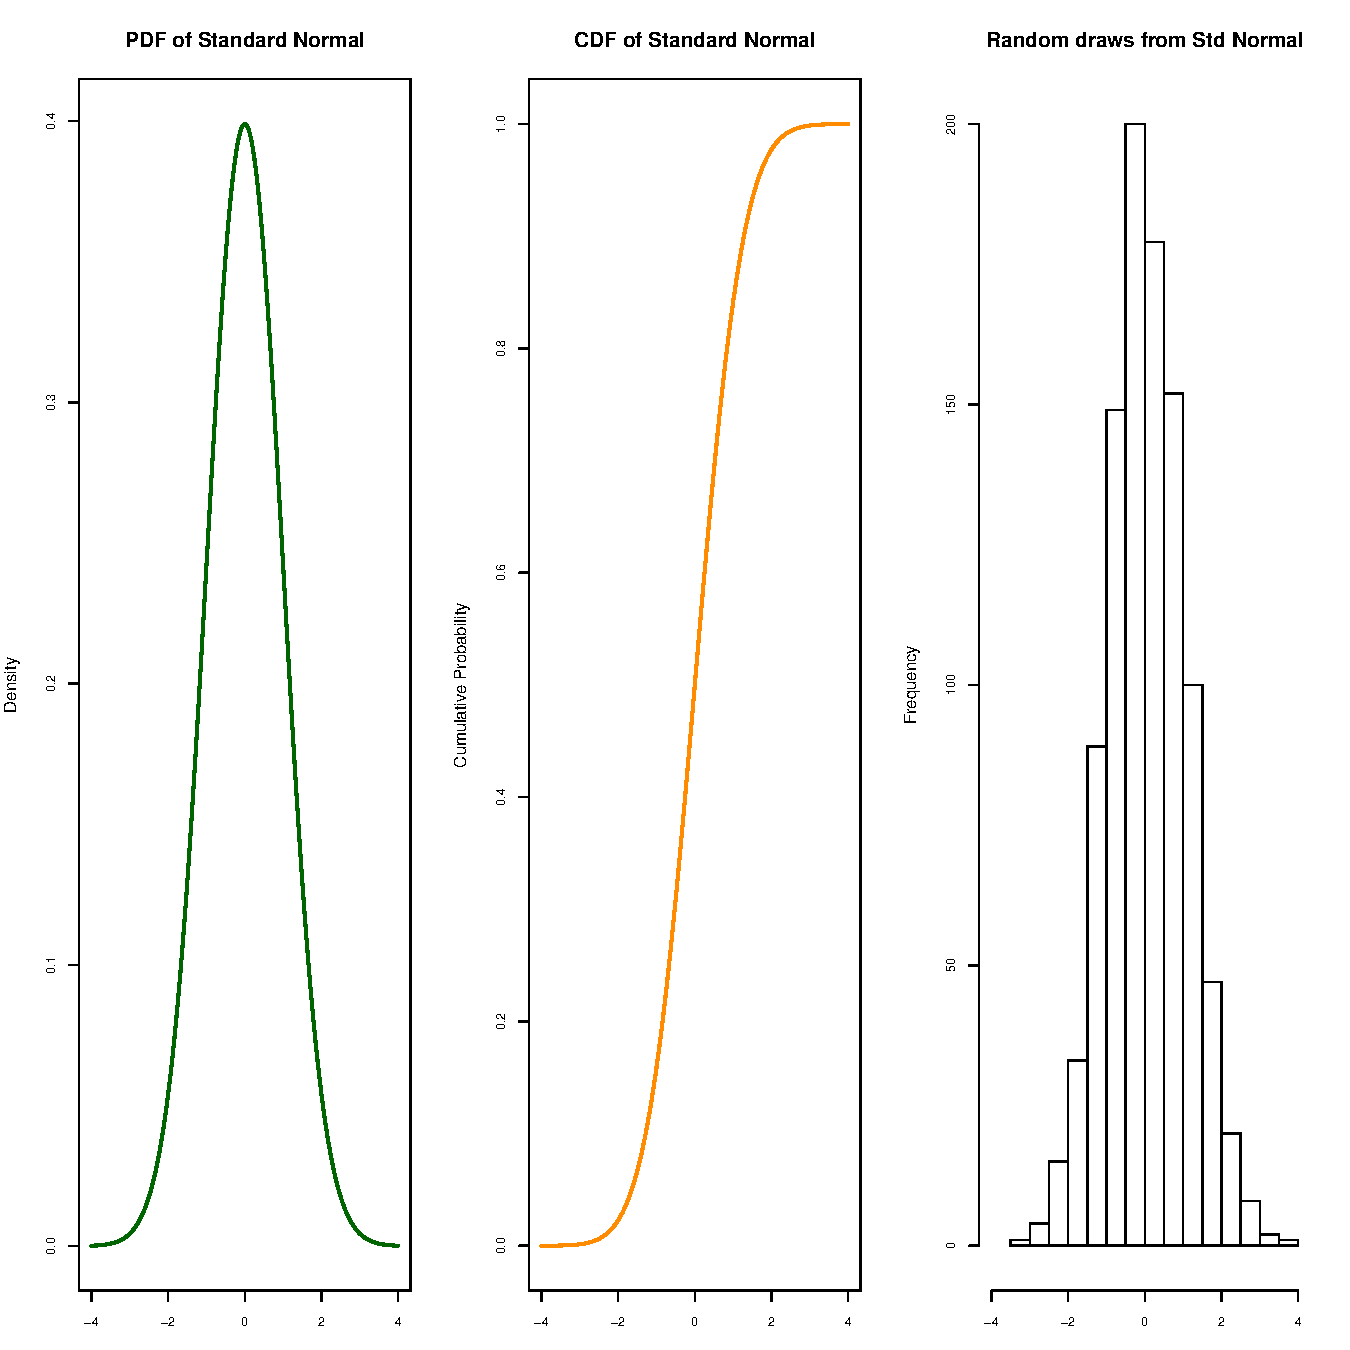
\includegraphics[width=0.9\linewidth,height=0.9\textheight,keepaspectratio]{/ifs/home/kellys04/AutoReportLite/analysis_pipeline/Sample4/Sample4.random_distribution.pdf}
\end{frame}

\section{Sample5}
\subsubsection{Stats}
\begin{frame}{Stats }
\small{
Sample5 

Some sample stats

[1] -4.00 -3.99 -3.98 -3.97 -3.96 -3.95

[1] 0.0001338302 0.0001392850 0.0001449476 0.0001508253 0.0001569256

[6] 0.0001632564

[1] 3.167124e-05 3.303665e-05 3.445763e-05 3.593632e-05 3.747488e-05

[6] 3.907560e-05

[1]  1.2582925  0.6447519  0.4633460  0.7703058 -0.2263347 -0.3515479
}

\end{frame}

\subsubsection{distribution\_histogram.pdf}
\begin{frame}{distribution\_histogram.pdf }
\scriptsize{/ifs/home/kellys04/AutoReportLite/analysis\_pipeline/Sample5/Sample5.distribution\_histogram.pdf}
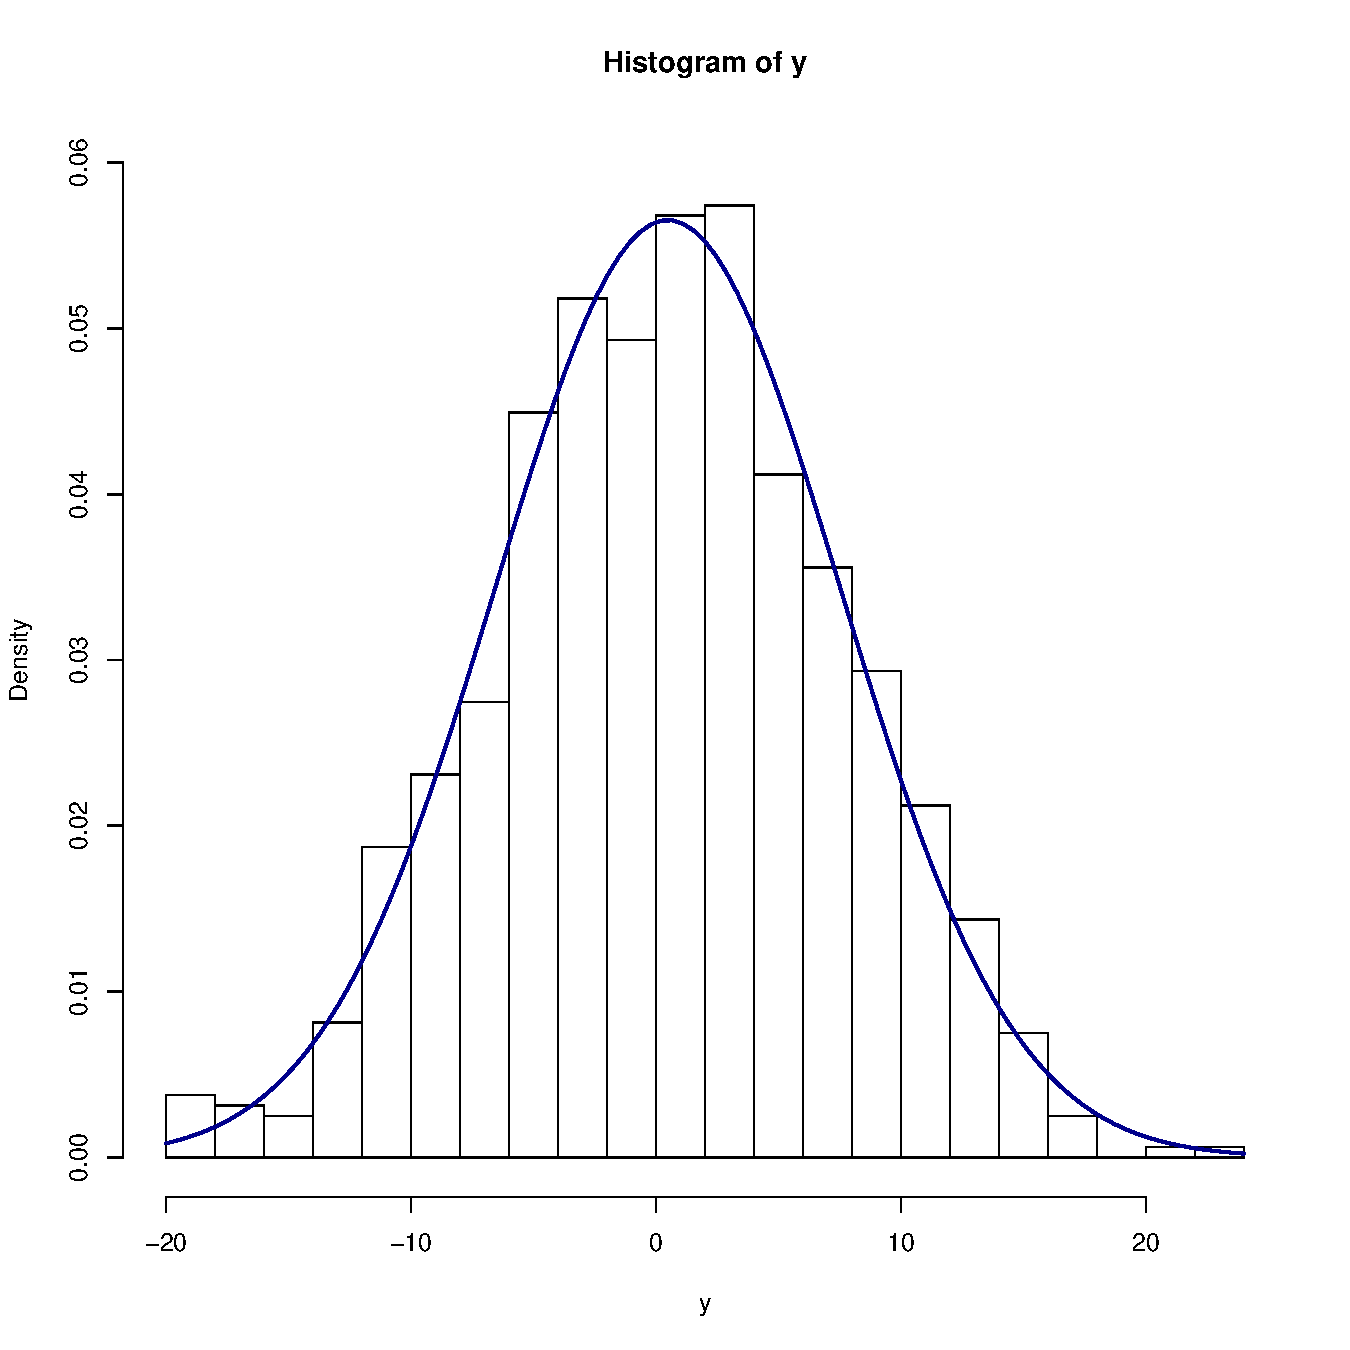
\includegraphics[width=0.9\linewidth,height=0.9\textheight,keepaspectratio]{/ifs/home/kellys04/AutoReportLite/analysis_pipeline/Sample5/Sample5.distribution_histogram.pdf}
\end{frame}

\subsubsection{random\_distribution.pdf}
\begin{frame}{random\_distribution.pdf }
\scriptsize{/ifs/home/kellys04/AutoReportLite/analysis\_pipeline/Sample5/Sample5.random\_distribution.pdf}
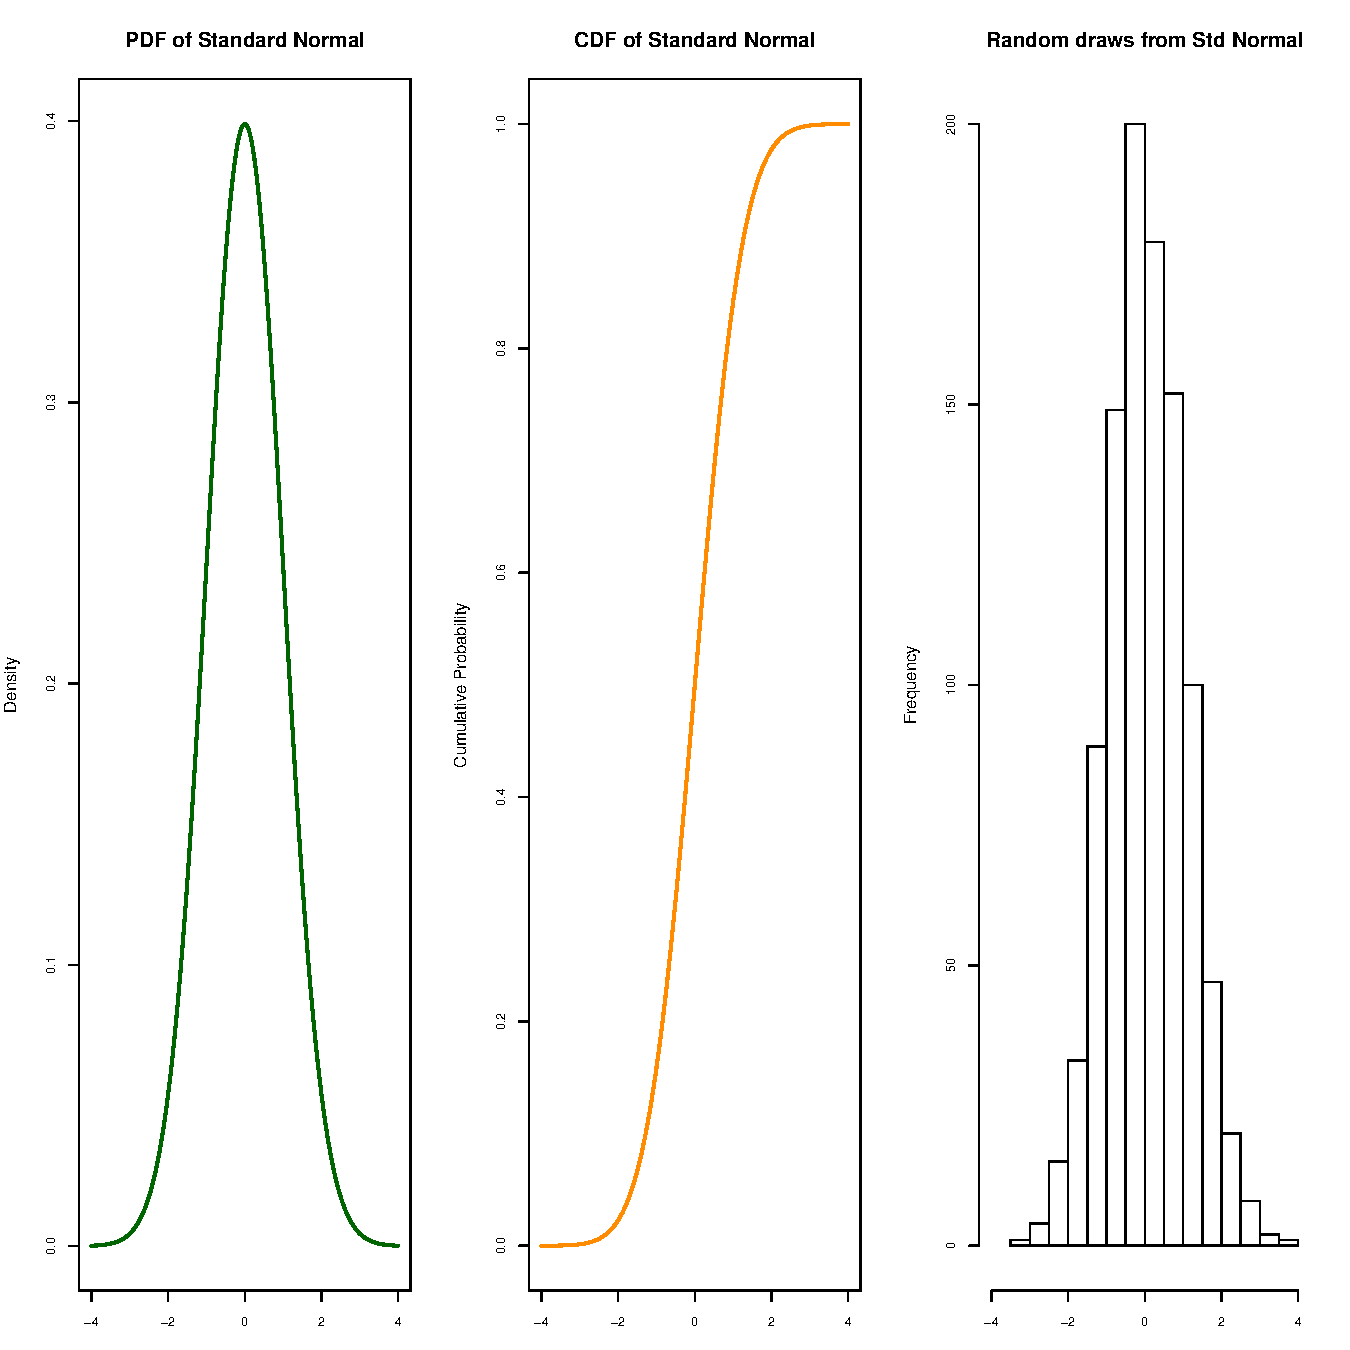
\includegraphics[width=0.9\linewidth,height=0.9\textheight,keepaspectratio]{/ifs/home/kellys04/AutoReportLite/analysis_pipeline/Sample5/Sample5.random_distribution.pdf}
\end{frame}



%%%%%%%%%%%%%%%%%%%%%%%%%%%%
\section{Session Information}
% \begin{frame}{System and Session Information}
% \begin{frame}[fragile]{System and Session Information}
\begin{knitrout}\footnotesize
\definecolor{shadecolor}{rgb}{0.969, 0.969, 0.969}\color{fgcolor}\begin{kframe}
\begin{alltt}
\hlkwd{system}\hlstd{(}\hlstr{'uname -srv'}\hlstd{,}\hlkwc{intern}\hlstd{=T)}
\end{alltt}
\begin{verbatim}
## [1] "Linux 2.6.32-573.18.1.el6.x86_64 #1 SMP Tue Feb 9 22:46:17 UTC 2016"
\end{verbatim}
\begin{alltt}
\hlkwd{sessionInfo}\hlstd{()}
\end{alltt}
\begin{verbatim}
## R version 3.2.3 (2015-12-10)
## Platform: x86_64-redhat-linux-gnu (64-bit)
## Running under: CentOS release 6.7 (Final)
## 
## locale:
##  [1] LC_CTYPE=en_US.UTF-8       LC_NUMERIC=C              
##  [3] LC_TIME=en_US.UTF-8        LC_COLLATE=en_US.UTF-8    
##  [5] LC_MONETARY=en_US.UTF-8    LC_MESSAGES=en_US.UTF-8   
##  [7] LC_PAPER=en_US.UTF-8       LC_NAME=C                 
##  [9] LC_ADDRESS=C               LC_TELEPHONE=C            
## [11] LC_MEASUREMENT=en_US.UTF-8 LC_IDENTIFICATION=C       
## 
## attached base packages:
## [1] stats     graphics  grDevices utils     datasets  methods   base     
## 
## other attached packages:
## [1] xtable_1.8-2    Hmisc_3.17-1    ggplot2_2.0.0   Formula_1.2-1  
## [5] survival_2.39-2 lattice_0.20-33 knitr_1.12.3   
## 
## loaded via a namespace (and not attached):
##  [1] Rcpp_0.12.3         cluster_2.0.4       magrittr_1.5       
##  [4] splines_3.2.3       munsell_0.4.2       colorspace_1.2-6   
##  [7] stringr_1.0.0       highr_0.5.1         plyr_1.8.3         
## [10] tools_3.2.3         nnet_7.3-12         grid_3.2.3         
## [13] gtable_0.1.2        latticeExtra_0.6-26 Matrix_1.2-5       
## [16] gridExtra_2.0.0     RColorBrewer_1.1-2  formatR_1.3        
## [19] acepack_1.3-3.3     rpart_4.1-10        evaluate_0.8.3     
## [22] stringi_1.0-1       scales_0.3.0        foreign_0.8-66
\end{verbatim}
\begin{alltt}
\hlkwd{save.image}\hlstd{(}\hlkwc{compress} \hlstd{=} \hlnum{TRUE}\hlstd{)}
\end{alltt}
\end{kframe}
\end{knitrout}
\LaTeX{} version: \LaTeXe~ \fmtversion
% \end{frame}
\end{document}
